\chapter{绪论} 
科学计算可以分为数值计算和符号计算两种. 数值计算的输入输出和中间结果都是数值, 因为计算机对数值的存储精度有限, 数值计算是一种近似计算. 而任意精度浮点数和有理数计算等精确计算都可以划分到符号计算的范围. 更加广义的符号计算指的是对代表数学对象的符号(包括整数\D 有理数\D 实数\D 复数\D 变量名\D 多项式\D 群\D 环\D 域\D 矩阵等)进行计算. 能够进行符号计算的软件也被称为计算机代数系统, 常见的计算机代数系统有Maple, Mathematica, Axiom, Maxima 和 Reduce 等. 计算机代数系统的出现, 对许多需要复杂的符号推理和计算的领域都提供了有力的工具. 尤其是在非线性系统的精确解的相关研究中, 计算机代数系统更是不可或缺的工具. 本文对于非线性系统精确解的相关研究, 都是基于 Maple 完成的. 

\section{非线性偏微分方程精确解的研究背景与相关工作}
非线性偏微分方程是描述自然界许多现象和内在规律的常用数学模型. 研究非线性偏微分方程精确解, 对我们了解事物的运动规律和科学地解释自然现象都起着重要的作用. 根据微分方程类型的不同, 构造精确解的方式也各不相同. 而非线性演化方程(Nonlinear Evolution Equations, 简称NLEE), 因为其形式较为简单且覆盖面广, 关于它的研究成果最为丰富. 

经过研究人员的不断努力, 发现了一些列具有普适性的求NLEE精确解的算法. 如反散射变换方法\cite{kawata1978inverse,ma2014verifying}\D Darboux 变换方法 \cite{matveev1991darboux,ling2018general,lou1997non}\D \Backlund{}变换方法 \cite{wahlquist1973backlund,li2008method,cheng2015multiple}\D 齐次平衡方法\cite{zhibin1993travelling,wang1995solitary,wang1996application,hbm1998,hbm1998b,hbm1999,senthilvelan2001extended,zhao2002new,feng2004comment,nguyen2015modified,rady2010homogeneous,eslami2014exact}\D Hirota 方法 \cite{hirota1971exact,hereman1991exact,hu2002application,hirota2003vector,ma2015lump}\D 混合指数方法\cite{hereman1986exact}\D 双曲正切方法\cite{huang1989exact,malfliet1992solitary,li_book_2007,parkes1996automated,li2002rath,fan2000extended,yan2001new,zheng2003generalized}\D Jacobi椭圆函数方法\cite{liu2001jacobi,zhang2003jacobi,zhou2003periodic,yin2002automated,yin2003automated,li2004raeem,chen2003improved,wang2005new,gui2005applications,chao2005symbolic}等. 基于这些方法能够得到许多不同类型的精确解, 如孤子解\cite{hirota1971exact,makhankov1980computer}\D 呼吸子解 \cite{tajiri1989breather,guo2011rogue,sun2018general}\D LUMP解\cite{satsuma1979two,villarroel1999discrete,imai1997dromion}\D 怪波解\cite{guo2011rogue,zhang2014rogue,sun2018general,zhaqilao2018symbolic}以及上述这些解的相互作用解等. 下面我们主要对齐次平衡方法\D 双曲正切方法\D Jacobi 椭圆函数方法和 Hirota 方法进行简要介绍. 

(a) 齐次平衡方法

1993年, 李志斌和王明亮\cite{zhibin1993travelling}提出了求解NLEE行波解的齐次平衡方法, 随后他们应用该方法求解了一系列方程\cite{wang1995solitary,wang1996application}. 齐次平衡方法将方程的解假设为关于某些函数的多项式之后, 通过平衡方程中最高次项的次数来确定解的次数, 再通过待定系数法进行求解. 因为它具有广泛的适用性, 所以他被国内外学者用于求解各种方程的精确解\cite{hbm1998,hbm1998b,hbm1999,senthilvelan2001extended,zhao2002new,feng2004comment,rady2010homogeneous,eslami2014exact,nguyen2015modified}. 因为齐次平衡方法具有广泛的适用性, 因此它也被提炼为齐次平衡原则, 在众多方法中发挥着重要作用. 如\Painleve{}分析\D 双曲正切方法\D Jacobi椭圆函数方法都用到了齐次平衡原则. 

(b) 双曲正切方法 

双曲正切方法始于黄国翔和楼森岳等人\cite{huang1989exact}的工作. 双曲正切方法将解假设为tanh函数的多项式, 基于齐次平衡原则确定解的次数之后, 再通过待定系数法求解. 1992年, Malfliet Willy \cite{malfliet1992solitary}系统地阐述了双曲正切方法. 1994年, 李志斌\cite{li_book_2007}年首次编写了基于双曲正切方法求解的非线性演化方程的程序, 并在代数方程的求解中引入了吴文俊消元法, 但是只能在交互的方式下完成方程的而求解. 1996年, Parkes EJ 和 Duffy BR \cite{parkes1996automated}基于Mathematica 编写了ATFM 软件包, 对于许多方程能够自动给出解。但是很多时候, 程序的运行还是需要人工干预, 并没有做到完全的自动化. 2002年, 李志斌和柳银萍\cite{li2002rath}在Maple 上编写了 RATH 软件包,完全自动地实现了双曲正切函数方法. 同时, 她还首次引入了一个变换, 可以在求得的双曲正切函数多项式的阶数不是正整数的时候对方程进行求解, 获得关于双曲正切函数的有理函数解. 同时, 范恩贵\cite{fan2000extended}\D 张鸿庆\D 陈勇\cite{zheng2003generalized}和闰振亚\cite{yan2001new}等人也对双曲正切方法进行了一些拓展和应用. 

(c) Jacobi椭圆函数方法

2001年, Liu Shikuo 等人\cite{liu2001jacobi}将双曲正切函数法中的 tanh 函数替换为 Jacobi 椭圆函数, 提出了求解 Jacobi 椭圆函数方法. 2003年, 张善卿和李志斌\cite{zhang2003jacobi}将该方法推广应用到一类新的 NLEE 上, 并获得了它们的精确周期解. 同年, 王明亮\D 周宇斌等\cite{zhou2003periodic}在 Jacobi 椭圆函数方法的基础上, 提出了F-展开法. 2002年,柳银萍和李志斌\cite{yin2002automated}研发了软件包 AJFM, 实现了 Jacobi 椭圆函数方法的完全自动化. 2003年, 他们\cite{yin2003automated}又研发了软件包 TRWS, 该软件包可以完全自动地推导出 NLEE 不同类型的行波解, 包括多项式解\D 指数函数解\D 三角函数解\D 双曲函数解\D 有理函数解\D Jacobi 椭圆函数解和 Weierstrass 椭圆函数解. 2004年, 他们\cite{li2004raeem}又研发了软件包 RAEEM, 解决了 TRWS 中的漏解问题, 并集成了软件包 RATH \D AJFM \D TRWS 的功能. 同时, 陈怀棠\cite{chen2003improved}\D 张鸿庆\cite{wang2005new}\D 徐桂琼\cite{gui2005applications} 和张解放\cite{chao2005symbolic}等人也对 Jacobi椭圆函数方法进行了拓展和应用. 

(d) Hirota 方法

Hirota 双线性方法是由日本数学家 Hirota 于1971提出的方法\cite{hirota1971exact}. 因其思路简单\D 适用范围广, 后被众多学者应用和推广. Hirota双线性方法首先在适当的变换下将原方程转化为双线性方程, 再将扰动展开式代入双线性方程中,在一定条件下将级数截断至有限项,最后构造出多孤立子解的表达式. 1973年, Hirota\cite{hirota1973exact}在求解浅水波的孤子解时, 将多孤子解生成公式重写, 该形式被后来的研究者们所广泛接受. 

基于 Hirota 方法不仅能够得到 NLEE 的多孤子解, 还能得到许多其他类型的解. 1979年, Satsuma J 和 Ablowitz MJ 在 Hirota \cite{satsuma1979two}方法的基础上提出了长极限方法, 解得了(2+1)KP\cite{kadomtsev1970stability}方程的LUMP解. 后来, 有许多研究者基于他们的方法得到了其它方程的LUMP解. 如 Gilson CR\cite{gilson1990lump}\D 马文秀\cite{ma2015lump,zhang2017lump,chen2018lump}\D 张岩\cite{ZHANG2018592,zhang2018m}\D Sun Hong-Qian\cite{sun2017lump}\D 和 Cheng Li\cite{cheng2017lump}等. 1989年, Tajiri M 等人\cite{tajiri1989breather}基于 Hirota 方法提出了共轭参数法, 能够从多孤子解得到呼吸子解. 1981年, Hirota 和 Ito \cite{hirota1983resonance}利用该方法得到了孤子方程的共振解. 1990年, Hietarinta \cite{hietarinta1990multidromion}利用该方法得到了 Davey-Stewartson 方程的 Multidromion 解. 1997年, Lambert F 等人\cite{gilson1996combinatorics,lambert1997construction,lambert2008soliton} 将 Bell 多项式和 Hirota 方法结合起来, 拓展了Hirota 方法的应用范围. Wazwaz AM 也\cite{wazwaz2008multiple,wazwaz2008integrable,wazwaz2009multiple,wazwaz20102,wazwaz2010multiple,wazwaz2012multiple} 对 Hirota 方法进行了许多的推广和应用. 范恩贵\cite{fan2011new}\D 胡星标\cite{hu1999soliton,hu2002application,hirota2003vector}和马文秀\cite{ma2011linear}等人也做了许多有意义的工作. 近年来, Hirota 方法还被用于求怪波解 \cite{guo2011rogue,sun2018general,zhaqilao2018symbolic}.

关于 Hirota 方法的机械化实现也有许多优秀的工作. 1992年, Hereman W 和 Zhuang W \cite{hereman1992symbolic,hereman1991macsyma} 简化了 Hirota 双线性方法, 提出了简单 Hirota 方法, 并在 Macsyma 上进行了实现, 该程序能够处理KdV型双线性方程. 2012年, 周振江\cite{zhou2012}在Maple上实现了 Hirota 双线性方法的相关软件包 Bilinearization 和 Multisoliton. 其中, Bilinearization 能够将 NLEE 双线性化, Multisoliton 能够求得多孤子解. 2014年, 张丽\cite{zhang2014}基于 Hereman W 和 Zhuang W 的工作, 在Maple上实现了简单 Hirota 方法的软件包 SHM. 此外, 还有杨云青和陈勇等人\cite{yang2011,miao2014pdebellii}在 Lambert F 等人工作的基础上, 结合 Hirota 方法和 Bell 多项式, 实现了 PDEBell 和 PDEBellII 软件包, 能够自动推导 KdV 类和 mKdV 类方程的孤子解. 

\section{非线性差分方程精确解的研究背景与相关工作}
求差分方程的精确解也是计算机代数的重要研究内容. 差分方程有时也被称为递归方程. 最简单的差分方程是线性常系数差分方程, 即
\begin{equation}
\sum_{k=0}^l{c_k f(x+k)}=g(x).
\label{ceq}
\end{equation}
其中, $f(x)$ 是未知函数, 而$g(x)$表示任意多项式, 而$c_k (k=1,\cdots,l)$是任意常数. 上述方程的求解在很久以前就已经被解决了. 而我们可以简单地将\refeqn{ceq}拓展为线性多项式系数的方程
\begin{equation}
\sum_{k=0}^l{p_k(x)f(x+k)=p_{l+1}(x)},
\label{peq}
\end{equation}
其中$p_k(x) (k=1,\cdots,l+1)$是多项式. 大概在30年前才首次出现对于该方程的研究. 在1989年, Abramov首先考虑了该方程, 并且提出了求解多有多项式解的算法\citep{Abramov1989polynomial}. 同年, Abramov 又提出了寻找所有有理函数解的公分母的算法, 从而提出求解所有有理函数解的算法\citep{Abramov1989rational}. 在1992年, \Petkovsek{} 提出了求解超几何函数解的算法\citep{petkovvsek1992hypergeometric}. 超几何函数相邻两项之比是有理函数. 在超几何函数解上进行移位和部分和操作能够生成 d'Alembertian 解. 而 d'Alembertian 解的求解算法是在1994年由 Abramov 和 \Petkovsek{} 共同提出的\citep{abramov1994dAlembertian}. 在 d'Alembertian 解上执行移位\D 部分和以及交错操作能够得到 Liouvillian 解. 而 Liouvillian 解的求解算法是在1999年由 Hendricks 和 Singer 提出的\citep{hendricks1999Liouvillian}.

\refeqnn{peq}的解的类型的拓展目前止步于 Liouvillian 解. 但是求解的算法还在不断改进. 一些改进是将这些算法推广到q-差分方程和微分方程. 例如\citett{Abramov1995polynomial}是对多项式解的推广应用, 而\citett{Abramov1995Rational} 是对有理函数解的推广应用. 另一些改进是为了提高算法的效率. 例如, \citett{ud2007,ud2010,ud2011,ud2012} 是一系列对有理函数解公分母的求解算法的改进. 这些改进极大的提高了有理函数阶的求解效率, 因为这一步是有理函数解求解过程耗时最长的一步. 

目前, 线性差分方程的研究成果较多, 而对于非线性差分方程的求解, 研究成果主要集中于几类特定的方程\cite{chen2011some,ishizaki2011difference}. 因此, 本文将对一般的非线性差分方程的精确解求解进行研究. 

\section{非线性积分化简的研究背景与相关工作}
在求微分方程精确解时, 往往离不开符号积分. 而符号积分也是计算机代数的重要组成部分之一. 关于基本初等函数的符号积分的研究开始于符号计算的发展初期. 最早的符号积分软件SAINT\spell{(Symbolic Automated INTegrator)}和SIN\spell{(Symbolic INtegrator)}分别发表于1963年\citep{slagle1963}和1967年\citep{moses1967}. 符号积分中最重要的基础算法是Risch算法\citep{risch1969,risch1970}, 它是近几十年来符号积分发展的基础. 在Risch算法发表后不久, Moses在SIN的改进版本中首次实现了纯超越函数的部分\citep{moses1971}. 而对于基本初等函数的一般情况, 是由Bronstein在1990年首次实现的\citep{bronstein1990}. 几乎所有的计算机代数系统(如 Maple, Mathematica, Axiom, Maxima 和 Reduce), 都是以Risch算法为基础来实现符号积分的计算的. 

当基本初等函数的符号积分被解决以后, 研究者们主要致力于特殊函数的符号积分的研究\citep{cherry1985,cherry1986,bertrand1994,jeffrey1997}. 近年来, 研究者们主要致力于特殊类型的积分, 如相对论库伦积分\citep{paule2012,paule2013}\D Feynman积分\citep{blumlein2012,smirnov2015}和参数积分\citep{raab2016}等.

然而, 关于抽象函数的积分的研究却很少. 只有文献\cite{deconinck2009}和文献\cite{poole2010}提出了一个算法来寻找线性可积的抽象函数表达式的积分. 他们的算法主要致力于寻找方程$D_x f=g$的解. 其主要作用是寻找偏微分方程中的守恒定律(conservation law)\citep{poole2011}, 而不是计算一般的抽象函数积分表达式. 因此, 本文将抽象函数积分的化简作为一个挑战性的课题进行研究, 并提出一个相应的算法.

\section{本文的选题和主要工作}
本文的主要工作分为非线性微分方程求解\D 非线性差分方程求解和非线性积分化简三个部分, 它们的逻辑结构如\reffig{outline}所示. 在\reffig{outline}中, 椭圆表示方法\D 矩形表示软件包. 其中, 软件包元素的第一行是软件包的名称, 第二行是软件包用途的简要说明. 软件包以4种颜色进行区分, 黄色表示基础工具, 蓝色表示用于求解差分方程, 绿色表示用于求解微分方程, 粉色表示用于进行积分化简. 即, 对于微分\D 差分\D 积分这三种不同的非线性系统的一些具体问题, 本文共实现了8个Maple软件包.

\begin{figure}[htbp]
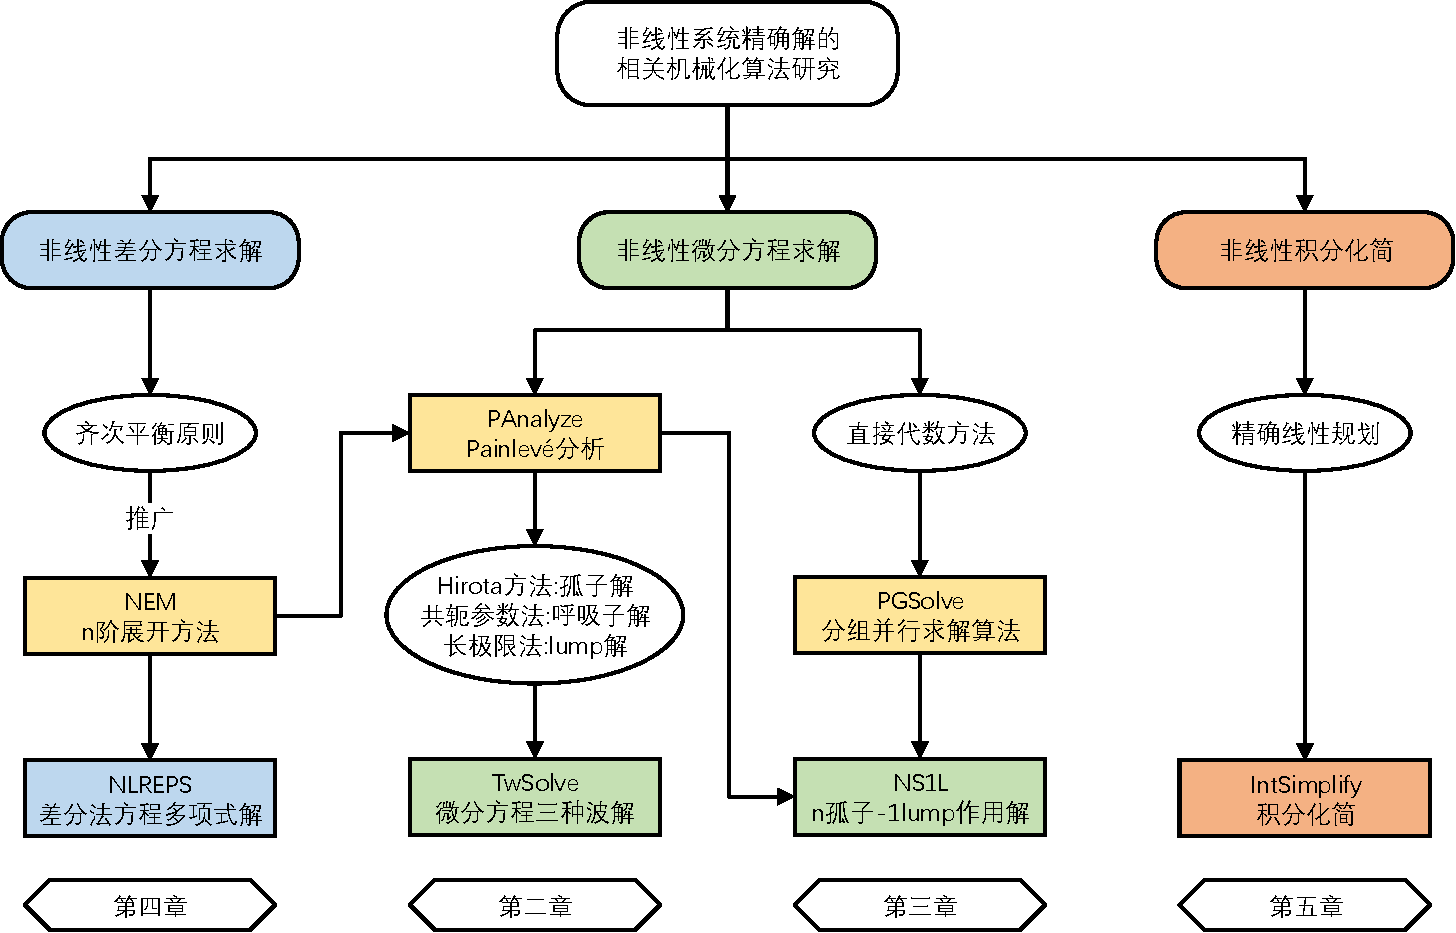
\includegraphics[width=\textwidth]{fig/outline.pdf}
\caption{本文工作大纲图}\label{outline}
\end{figure}

在\refchp{ch02}中, 本文以 \Painleve{} 分析和简单 Hirota 方法为基础, 实现了非线性演化方程三种波解的求解. 其中, 孤子解通过简单 Hirota 方法获得. 获得孤子解之后, 可以通过共轭参数法得到呼吸子解, 通过长极限法得到LUMP解. 本文将上述求解过程打包在TwSolver软件包中. 本文的工作不是对已有的方法进行简单的整合, 而是将 Hirota 方法推广到不可积方程并对编程实现进行优化, 是的我们的程序对于$n+1$维的NLEE能够求得满足原方程的真解. 

直接代数方法在微分方程求解中也有广泛的应用, 但其往往伴随着大规模代数方程组的求解. 在\refchp{ch03}中, 本文针对大规模代数方程组求解困难的问题, 设计了一个分组并行求解的算法, 并将其实现为 PGSolve 软件包. 作为PGSolve的应用实例, 本文开发了用直接代数方法求$n$-孤子和1-LUMP相互作用解的软件包 NS1L. 

在\refchp{ch04}中, 受到在微分方程求解中被广泛应用的齐次平衡原则的启发, 本文将其用于求解非线性差分方程的多项式解. 齐次平衡原则通过平衡方程中最高次项的次数来确定解的次数, 只能在一些情况下生效. 本文考虑同时平衡方程中最高$n$项的次数和系数, 提出了$n$阶展开方法来处理齐次平衡原则不能处理的情况, 并将其实现为一个便于拓展应用的软件包 NEM. 基于NEM, 实现了能够求解非线性差分方程所有多项式解的软件包 NLREPS. 

在微分方程的求解中, NEM 能够快速地完善基于齐次平衡原则的求解算法. 在\refchp{ch05}中, 我们以双曲正切方法为例, 基于 NEM 重新实现了一个 NTCM 软件包. 该软件包在将双曲正切方法推广到$n+1$维的同时, 利用NEM在阶数分析上的优势, 求解了许多以往不能求解的方程. 同时, 我们也以 \Painleve{} 分析为例展示了 NEM 的作用. 

在\refchp{ch06}中, 因为在非线性微分方程求解的过程中往往需要进行非线性积分表达式的化简, 本文将非线性积分化简作为一个具有挑战性的任务进行研究. 首先, 本文建立了一个代数系统将关于抽象函数的积分多项式视为标准积分项的线性组合. 然后, 基于导数的乘法规则, 设计了一个递归算法来寻找所有的二项合并规则. 最后, 基于这些规则将化简问题转化为一个精确线性规划问题进行求解, 实现了非线性积分表达式化简的软件包 IntSimplify. 

\refchp{ch07}对本文完成的工作进行了总结与讨论,概括了本文的主要研究方法和结论,并提出了对未来工作的展望.
